
\section{Styrenhet}

Styrenheten har till uppgift att driva de motorer som driver hjulen och de servon som styr armen.

\subsection{Framdrivning}

Motorenheten innehåller två hjulpar, de styrs separat för att göra det möjligt att svänga. Huvudmodulen skickar kommandon för hur snabbt vardera hjulpar skall rotera, styrenheten ser sedan till att motorerna kör i den efterfrågade hastigheten. Detta sker dock utan någon återkoppling från den verkliga hastigheten utan vi mäter upp vilken signal till motorerna som ger vilken hastighet och sedan används detta för att styra hastigheten under användning.

\subsubsection{Arbetsblock}
\begin{itemize}
\item Ta emot kommandon från huvudmodulen om vilken hastighet båda hjulparen ska hålla
\item Omvandla hastigheten till lämpliga PWM signaler
\item Starta motorn mjukt 
\item Lägg PWM signalerna på motorernas utgångar 
\item Stanna motorn mjukt
\end{itemize}

\subsection{Robotarm}

Robotarmen består av 7 servon av modell AX12-A. Dessa styrs genom att en målvinkel sätts (0-1023), med möjlighet att ändra hastighet, vridmoment och styra av/på. Från huvudmodulen får enheten målvinklar för varje enskild led. Styrmodulen är ansvarig för att se till att parallella servon körs synkroniserat, för att inte slita sönder varandra. Styrmodulen ansvarar också över att armen inte ska kollidera med resten av roboten. Den kommer att programmeras med vilka rymdmängder som den ej får passera och om den får kommandon som gör att den kommer passera dessa mängder måste den välja en annan väg än rakaste vägen.  
\newline
\centerline{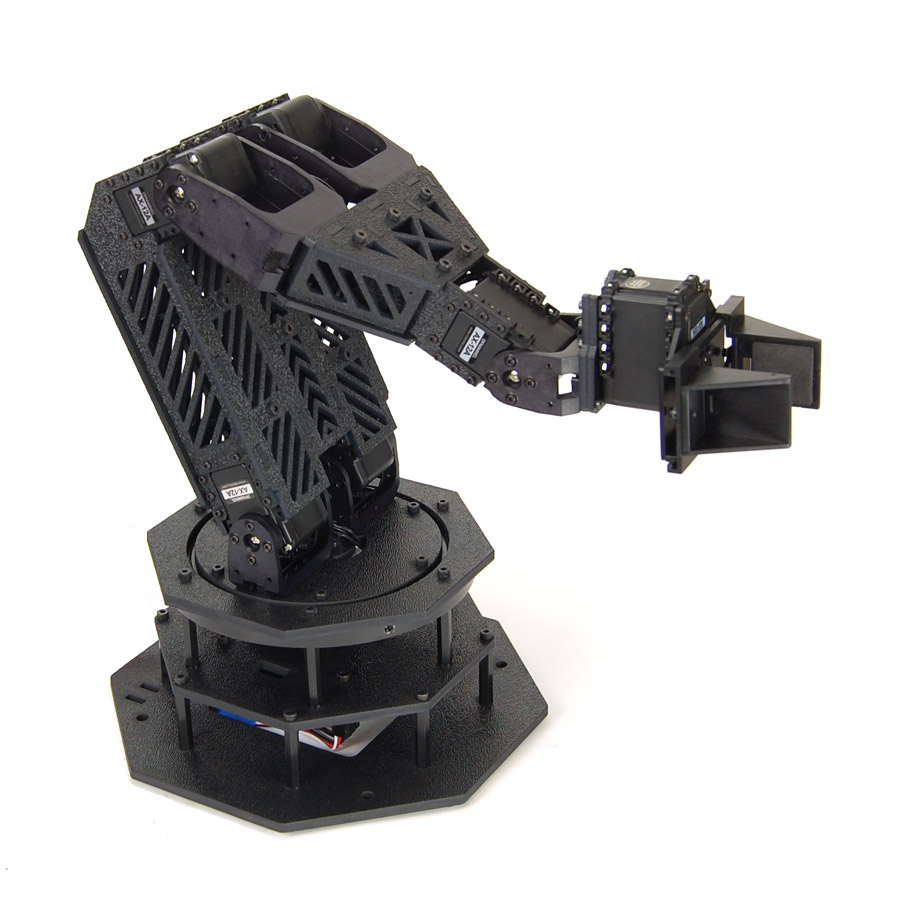
\includegraphics[scale=0.4]{arm}}


\subsubsection{Arbetsblock}

\begin{itemize}
\item Ta emot kommandon från huvudmodulen om vilka vinklar alla servon ska ha
\item Kolla om armen kommer röra sig igenom förbjuden rymd och beräkna en alternativ väg
\item Skicka kommandon till servona och se till så att de rör sig mjukt
\end{itemize}

\subsection{Processor}

Eftersom motorenheten kommunicerar med huvudmodulen genom UART kommer kommandon att tolkas med avbrott. Förslagsvis ska en Atmega16 microcontroller användas.